\documentclass[border=4pt]{standalone}

\usepackage{tikz}

\definecolor{otblue}{HTML}{0072B2}
\definecolor{otorange}{HTML}{E69F00}
\definecolor{otteal}{HTML}{009E73}
\definecolor{otpurple}{HTML}{CC79A7}
\definecolor{otgray}{HTML}{5A5A5A}

\begin{document}
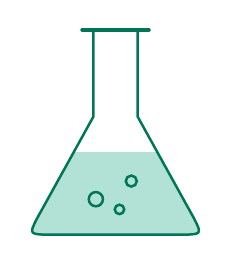
\begin{tikzpicture}[line width=0.9pt]
  \begin{scope}
    \clip (0.72,2.6) -- (0.72,1.5) -- (0,0.2) .. controls (-0.1,0) .. (0.2,0) -- (1.8,0) .. controls (2.1,0) .. (2,0.2) -- (1.28,1.5) -- (1.28,2.6) -- cycle;
    \fill[otteal!30] (-0.2,0) rectangle (2.2,1.05);
  \end{scope}
  \draw[otteal!75!black, line join=round] (0.72,2.6) -- (0.72,1.5) -- (0,0.2) .. controls (-0.1,0) .. (0.2,0) -- (1.8,0) .. controls (2.1,0) .. (2,0.2) -- (1.28,1.5) -- (1.28,2.6);
  \draw[otteal!75!black, line width=1.6pt, line cap=round] (0.58,2.6) -- (1.42,2.6);
  \foreach \x/\y/\r in {0.75/0.45/0.09,1.2/0.68/0.07,1.05/0.32/0.06}{\draw[otteal!75!black] (\x,\y) circle[radius=\r];}
\end{tikzpicture}
\end{document}
